\documentclass[a4paper]{howto}

% BIG FAT NOTICE: I hacked verbatim.perl to avoid it wrapping my
% verbatiminputs in <BR>s (no idea why it does that). The diff is as
% follows:
%
% --- verbatim.perl.orig  Sat Oct 12 14:14:15 2002
% +++ verbatim.perl       Sat Oct 12 14:14:17 2002
% @@ -110,7 +110,7 @@
%         $env_id .= ' CLASS="verbatim"' unless ($env_id =
% /(^|\s)CLASS\s*\=/i);
%         $verb_pre =~ s/>/ $env_id>/;
%      }
% -    join('', $closures, "<BR>\n", $verb_pre
% +    join('', $closures, "\n", $verb_pre
%         , $verbatim_mark, 'verbatim', $global{'verbatim_counter'}
%         , '#', $verb_post, $reopens, $outer);
%  }
%
% Generating docs without this mod will cause verbatim stuff to look
% like crap, you have been warned.
%
% Oh, and the image scales are correct. Don't mess with them, it takes a
% lot of time to discover the right ones. And yes, I copy over the
% original pngs over the generated ones; look at the Makefile.

\usepackage{verbatim}
\usepackage{graphicx}

\title{Developing applications with Kiwi}

\release{1.9.28}

\author{Christian Reis\\Johan Dahlin\\Async Open Source, Brazil}
\authoraddress{kiko@async.com.br\\jdahlin@async.com.br\\http://www.async.com.br/projects/kiwi/}
\date{August, 2006}

\begin{document}
%\maketitle

\begin{abstract}
\noindent
{\bf Kiwi is a library designed to make developing graphical
applications as easy as possible}. It targets developers that work with
{\bf Python} and that are looking for a way to produce applications with
good design without a lot of bureaucracy.  It offers both a framework
and a set of enhanced widgets, and is based on Python and PyGTK. Kiwi
borrows concepts from MVC, Swing and Microsoft MFC, but implements a set
of unique classes that take advantage of the flexibility and simplicity
of Python and GTK+ to make real-world application creation much easier.
In practice, code using Kiwi will be shorter, simpler and easier to
maintain than raw PyGTK, and just browsing through the examples in this
guide and in the package should give you a good idea of how.

{\bf Kiwi includes a framework and a set of enhanced widgets}. There is
\citetitle[http://www.async.com.br/projects/kiwi/api/]{complete API
documentation} to accompany the library, and this paper covers the
Framework in detail, providing examples, screenshots and advice on
designing your application.

All you need to use Kiwi is Python and PyGTK. Gazpacho is a useful add-on,
and is strongly recommended. Kiwi's free software licensed under the LGPL
and can be used and embedded in any application.
\end{abstract}

\section{Kiwi: An Overview}

\textbf{Kiwi} is a Python module for developing graphical applications.
While most free software projects that support programming of graphical
interfaces concentrate on low-level infrastructure and components, Kiwi
provides a high-level framework that helps developers organize their
code and develop applications quickly, removing the need to do a lot of
low-level work to get basic functionality implemented. The framework
allows you to easily write applications that look like this:

\begin{center}
\includegraphics[scale=0.626]{images/diary.eps}

\small{(This example application, \file{examples/framework/diary/diary2.py}, has
65 lines, not counting the XML specification)}
\end{center}

\subsection{Introduction}
For many platforms, graphical applications are developed based on an
application framework that is provided by the platform. For Java we have
Swing (and AWT); for Windows we have MFC (and a number of others). In
general, these frameworks include a set of widgets that are used
natively.

James Henstridge's
\citetitle[http://www.pygtk.org/]{PyGTK}, an excellent
set of \citetitle[http://www.gtk.org/]{GTK+} bindings for
\citetitle[http://www.python.org/]{Python}, supports graphical programs
written in Python, but it offers only a set of widgets, not a framework;
you have to do all the work of organizing your application yourself.
{\bf Kiwi wraps PyGTK to offer both a framework to organize your
application, and a set of enhanced widgets} that can be used either from
the framework or directly in your application. You can use as much or as
little of it as you like.

A framework (in the object-oriented programming sense) is a set of
general purpose classes that work together to provide a base upon which
an application is built. Kiwi is a white-box framework; to use this type
of framework, you inherit and customize one or more classes, instantiate
them, and run it. In Kiwi, a high-level class that controls a window,
for instance, is called \class{BaseView}, and it provides a method
called \function{show\_and\_loop()} that renders it and starts the event
processing upon which all GTK+ (and therefore Kiwi) applications are
based.  The Kiwi framework includes a number of classes that can be
adapted to your specific needs, and they are described further in the
next section.

Kiwi is based on the real-world experience of using Python and GTK+
(through PyGTK) to develop a fairly large application,
\citetitle[http://www.stoq.com.br/]{Stoq}, which uses many concepts
common to most graphical applications: multiple windows and dialogs,
forms, data persistence, lists and high-level classes that support
domain objects directly.

\subsection{Why Use Kiwi?}

You should use Kiwi if you develop a graphical software application
where Python is an option. Python is in my opinion the nicest of
the popular high-level languages available today, and I honestly
recommend all new applications be developed in a high-level language
for many reasons; ease of maintenance, speed of implementation and
security being the most important in my experience.

Kiwi implements a number of interesting tweaks to the standard MVC (or
MV+C) architecture, which is the base of most application frameworks
that exist out there, and a lot of research has gone into the framework
and the widgets to make development as convenient as possible. It goes
way beyond providing a basic `document plus view' schema, doing widget
conversion, automatic signal connection, and adjusting behavior
automatically to reduce drastically the amount of code needed to define
the windows and dialogs for your application. Kiwi also includes native
gtkbuilder support, which allows you to graphically specify (using glade)
your user interfaces and use them seamlessly as part of the framework.

The code used in Kiwi has been developed with quite a lot of care, and
though it is complex in parts (even crufty in a few spots), we consider
it to be generally easy to understand and change, and you can hijack and
customize the code to your need if you feel you don't want YAD (yet
another dependency) for your application.

Kiwi is also being actively developed and supported as a building block
in Stoq, and over the past years has grown to become very useful.
We welcome feedback and have been very fast to respond to requests and
bug reports, so you can be sure your application will be relying a
library that is actively supported and that its authors have a
continued interest in maintaining.

\subsection{Getting and Installing Kiwi}

Kiwi is distributed through its official website, at
\url{http://www.async.com.br/projects/kiwi/}. It is released as a
tarball frequently, and the tarball is distributed from that page.
Announcements of the release should go out to \code{pygtk-list},
\citetitle[http://freshmeat.net/]{Freshmeat} and \code{python-announce}.

You will need to install the following packages if they are not
already on your system:

\begin{itemize}
  \item  \citetitle[http://www.python.org/]{Python} 2.3 or newer
  \item  \citetitle[http://www.gtk.org/]{GTK+} 2.8
  \item  \citetitle[http://www.pygtk.org]{PyGTK} 2.8
\end{itemize}

Most of these packages are available on the main distributions,
including Fedora, Ubuntu, Debian, Conectiva and Mandrake, and might even be
preinstalled in your system. If not, you can pull the source code,
compile and install them.

% XXX: Add subversion checkout instructions
You can also use SVN to check out Kiwi, by following the instructions on
the \citetitle[http://www.async.com.br/projects/cvs.php]{Async CVS
page}. The module name is \code{kiwi}.
\citetitle[http://svn.async.com.br/cgi-bin/viewcvs.cgi/kiwi/?view=query&dir=&file=&file_match=exact&who=&who_match=exact&querysort=date&hours=2&date=month&mindate=&maxdate=]{Async's
ViewCVS service} can be used to check development of the kiwi module in
real time, and there is also an
\citetitle[http://svn.async.com.br/cgi-bin/viewcvs.cgi/]{browse source} of the code.
Finally, bugs in kiwi should be reported to
\citetitle[http://bugs.async.com.br/]{Async's installation of Bugzilla}.

Kiwi includes a fair amount of tests in the \file{tests/} directory in
the tarball, and they can be run in-place (no need to install it first),
so you can easily see what sort of application it supports.

Since Kiwi uses Distutils, installing Kiwi should be very simple.  Once
you have installed the dependent packages, run (as root, normally):

% XXX: --prefix and non root installation

    \begin{verbatim}
    python setup.py install
    \end{verbatim}

in the main directory. That's it. To test the installation, do:

    \begin{verbatim}
    >>> import kiwi
    \end{verbatim}

from the Python console. It should work, and if it does, everything
is ready.

\section{The Kiwi FrameWork}
\label{person}

This section introduces the Kiwi framework, and shows the use cases that
each of the main classes were designed for. Throughout this guide, I'll
be showing code examples that are included in the distribution (in the
\file{examples/} directory); just install Kiwi and you are ready to run
them. To start off with, I'll show a very simple Kiwi application that
saves information defined in a graphical form. This app is included in
\file{examples/framework/person/person.py}.  Note that this app uses the
glade file \citetitle[Person.glade]{Person.glade}.

\begin{center}
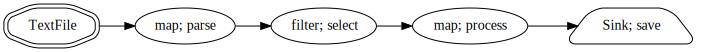
\includegraphics[scale=0.905]{images/simple.eps}
\end{center}

\verbatiminput{../examples/framework/person/person.py}

This application (17 lines) renders an interface to edit personal data,
transparently saving and loading it. A quick glance at the code:

\begin{enumerate}
\item We define Person, a class to hold our application information
\item \code{Person.unpickle()} loads (creating, if it didn't exist) a
Person instance.
\item We create a \class{ProxyDelegate} instance, which loads an interface
from a glade definition file and attaches it to the Person instance.
\item We run the application; changes in the interface reflect
transparently on the person instance.
\item Upon exiting the mainloop, the window closes and we save the
person. It is ready to be edited the next time we run the program.
\end{enumerate}

This example is a summary of many Kiwi features; it exemplifies the
Proxy class, which is one of the more featureful parts of the
framework. This guide will take you gradually through the different
classes in Kiwi, and the next section begins by describing the general
Kiwi architecture.

\subsection{Introduction}

The Kiwi framework is based loosely on two important concepts.

\begin{enumerate}
\item The first concept is Model-View-Controller (MVC), which is an
architecture developed for Smalltalk and that has been discussed and
reused many times before (there are some references at the end of the
text if you are curious about it). I have done some study of
MVC\footnote{ While MVC is both interesting and commonplace, I criticize
it as a generic solution to an application-level framework because it
tends to promote highly-coupled classes (it does work quite nicely as a
widget-level framework, having said that).
Of course, this doesn't mean it's not useful to many applications (or at
least parts of them).} and MVC implementations in modern frameworks
(Swing and MFC both implement MVC in their own ways), and Kiwi provides
traditional Views and Controllers (V and C) as well as Delegates, which
are combined Views and Controllers (using the same name as under Swing).

\item The second concept is the Proxy, which borrows somewhat from Allen
Holub's `visual proxy' concept described in his series
\citetitle[http://www.javaworld.com/javaworld/jw-07-1999/jw-07-toolbox\_p.html]
{Building user interfaces for object-oriented systems}. Allen's views
are quite original and gave a lot of insight into what coupling really
meant for graphical interfaces.

The visual proxy is an object that represents a model, or a certain part
of it. It is coupled to the model it represents, which isn't absurd
taking into account that it is simply a way to view and change it. In
Kiwi you use Proxies in combination with Delegates (or separate Views
and Controllers) to build forms for applications.
\end{enumerate}

\subsection{The FrameWork Classes}

The Kiwi framework is made up of a set of classes and some helper
functions that are used to define the behavior of your application.
The Kiwi classes are organized into the following groups:

\begin{itemize}
\item \class{Views}, which represent the graphical display; a View defines
an interface's widgets and their layout.
\item \class{Controllers}, which handle signals generated by the user
interacting with the widgets in a View.
\item \class{Delegates}, which are classes that combine the features of
a View and a Controller.
\item \class{Models}, which are mixins your domain object can
inherit from to take advantage of special functionality.
\item \class{Proxies}, special types of Delegate designed to implement
forms. Proxies attach themselves to an instance, and transparently
modify this instance as the user interacts with the widgets in its
interface.
\end{itemize}

Of these, \class{Controllers} and \class{Models} do not implement user
interfaces themselves, and are used together with one of the different
user interface (UI) classes.

{\bf A special note:} When using a white-box framework, it is very
important to take care when defining names in the inherited classes to
avoid clobbering names defined in the base classes you inherit from. It
is useful to read through the
\citetitle[http://www.async.com.br/projects/kiwi/api/]{API
documentation} and check for naming conflicts, and to understand which
hooks might be interesting to reimplement. If you find something in your
code is behaving very strangely, this could be one of the first things
to check.

\subsection{Views}

A View is a class that defines how a single window will look.
Differently from most frameworks, Kiwi requires almost no infrastructure
code to create a trivial app; Kiwi allows you to create a view and run
it by itself, with no attached handlers, controller or model. (Whether
or not this is a very useful app is another matter, but let's get you
started on it before you criticize me.)

There are a number of different Views available for Kiwi, which live in
the \module{kiwi.ui.views} module:

\begin{itemize}
\item \class{BaseView}, which is a View with a toplevel window, in which
you create and organize the widgets using PyGTK classes and commands.
\item \class{BaseView}, which allows widgets to be defined using Glade
and loaded in runtime using gtkbuilder or libglade. This allows widgets to
be easily changed and rearranged visually, without the code needing
to be changed.
\item \class{SlaveView}, which is a View with a toplevel widget that is
not a window. SlaveViews are designed to be embedded into other Views,
usually representing a part of an interface that must be reused in
multiple places in your application. Kiwi makes it easy to reuse that
complicated form that you created in multiple windows of your app.
\end{itemize}

To start off, the easiest way to demonstrate a View is to create a very
simple one that does nothing but present a fixed label on the screen.
This first example will use GTK+ widgets directly, just to show how they
fit in (it's available in the Kiwi tarball in
\file{examples/framework/hey/hey.py}).

\begin{center}
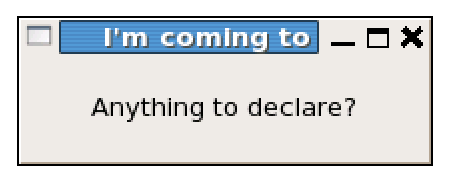
\includegraphics[scale=0.905]{images/london.eps}
\end{center}

\verbatiminput{../examples/framework/hey/hey.py}

So what does the example do? To start off with, it defines a view class
that inherits from \class{BaseView}, the View with a toplevel window.
BaseView should always be subclassed, since it requires you to to create
the widgets programatically.  You should instantiate and assemble PyGTK
widgets in the constructor before running
\function{BaseView.\_\_init\_\_()}. We initialize \class{BaseView} with
two parameters\footnote{Note that I used positional parameters here just
to make things clear; they are in the proper order and the whole call
could be \code{Views.BaseView.\_\_init\_\_(self, win, gtk.main_quit)}.}

\begin{itemize}
\item \function{toplevel}, which defines which widget is the toplevel
widget for that view. For a BaseView, this is the window you want to
display. We pass in the gtk.Window we just created. The toplevel widget
is used for setting focus and showing the View.
\item \function{delete\_handler}, which defines which function should be
called when the window is deleted (this happens when the almost ubiquitous "X"
button offered by window managers is clicked, or \code{del(window)} is
invoked). We are passing in gtk.main.quit, which breaks the main loop we are
running in, and allows the application to exit. Note that we're passing
in the function object itself, instead of the result of a function call.

If you didn't pass in a delete handler, closing the window would leave
the python interpreter hung in the mainloop. What mainloop? Read on.
\end{itemize}

Right after we instantiate our view class, we call a special method in
it: \code{show\_and\_loop()}. This method calls show() on all the
widgets under the toplevel widget including it (in our cases, it will
show the label and the window), and runs the GTK+ event loop (or
mainloop). The mainloop is a fundamental aspect of GUI programming: when
it is invoked, it assumes control of the normal flow of execution and
continuously processes events that are generated by user interaction
with the widgets. You can read more about the mainloop in the mainloop
section of
\citetitle[http://developer.gnome.org/doc/GGAD/sec-mainloop.html]
{GTK+/Gnome Application Development}.

Right now, the relevant aspect of the mainloop is that we will need to
break this loop when we quit our application, which for this app should
happen when you click on "X". This is why we are passing in
\function{mainquit} as \code{delete\_handler}: to stop the mainloop and
let the control go back to our code (which also ends right after, at
which time you are left staring at the console).

\class{BaseView} is the most basic type of view, and it's only worth so
much explaining. The next section describes \class{BaseView}, which is
a lot more interesting.

% ====================
% ====== MARK ========
% ====================

\subsection{BaseView}

Once you have written three (two?) applications using the PyGTK classes
and commands directly, you get very bored of hand-coding the widgets and
their structure. Sure, you have total control over them, and you can
build them programatically, which is why you {\it might} want to do it
for small parts of your application, but for anything that is medium to
large-scale, having to maintain all that code makes changing the UI very
painful. Damon Chaplin's application
\citetitle[http://glade.gnome.org/]{Glade} provides a way to create a
GTK+ interface visually, and it is normally used to generate C or C++
code that creates the widgets. It also saves the interface specification
in an XML file. Knowing this, James Henstridge, the author of PyGTK,
wrote libglade, a killer library (this was years ago, but I digress)
that renders widgets based on specifications in an XML file. libglade
allows you to keep the interface definition separate from the code,
which is an awesome idea, since it drastically reduces the amount of
interface code (and the consequent burden of maintaining it). Being able
to use Glade to revisit and tweak your interface without having to
regenerate code is also a huge advantage.

Anyway, Kiwi lets you use Glade interfaces in a {\bf very} convenient
manner, by using the \class{BaseView} class. Let's show this off by
redoing the last example using glade. First thing would be running Glade
and creating a window and putting a label into it. Name the window
\code{hey} and turn the visible property off (using the Common tab of
the Properties dialog). Save the file (careful with that Save dialog, it
creates directories and is generally evil in my opinion) as
\file{hey.glade}. And then code up \code{heyglade.py} (all this is
available in \file{examples/framework/hey/heyglade.py}):

\verbatiminput{../examples/framework/hey/heyglade.py}

Oops. Where did all that code go? Right, we are now using the glade file
to generate the UI. So we didn't even need to subclass
\class{BaseView}; we just passed in a parameter that told it what glade
file to use, and the same delete handler. Note also that we used
\code{show\_and\_loop()} instead of
\code{show\_all\_and\_loop()}\footnote{ It is important to note that
BaseView does *not* allow you to call \code{show\_all\_and\_loop()} ---
you must use \code{show\_and\_loop()} instead.  There is a reason for
this. show\_all means that all widgets under the toplevel widget should
be shown; however in glade, since most widgets are visible by default,
you only need to turn off visibility on the toplevel window to get the
default hidden effect. This alone would not be a problem, but the fact
is that certain widgets can be configured in glade to *require* being
hidden (either because you want them initially hidden, or because they
do something special, like the gtk.Toolbar: if you choose to use `Only
Text' or `Only Icons', glade implements this by hiding the icons or
text, respectively). This would break with show\_all and too many bug
reports told me it was enough reason to turn it off. You can of course
call it manually on the window if you are really determined do so.}.

The \code{gladefile} parameter indicates the file it should open. If the
name you pass in doesn't have a \file{.glade} suffix, \class{BaseView}
will append it and try to open it; in our cases, it will try to open the
file \file{hey.glade}.  However, this argument does a bit more than just
specifying the file (when using this form of the constructor, which is
simplified): it also specifies by default the {\bf name of the toplevel
widget} in the glade file. This is why I specifically stated the window
should be named \code{hey} two paragraphs back. That widget is attached
to the view instance with the name \code{toplevel}.

If you want to use another specific toplevel widget name, just use the
extra constructor parameter \code{toplevel\_name}. This can be useful
if you have many windows in the same Glade file; you can reuse the glade
file by just defining multiple \code{BaseView} instances (or subclass
instances) with the same \code{gladefile} but specifying different
toplevel widgets as each individual \code{toplevel\_name}.

There are some common mistakes to be made when using the BaseView, and
Kiwi raises special exceptions for three them.

\begin{enumerate}
\item The first one is forgetting to specify the gladefile, or giving it
the wrong name. Kiwi will try to look for the file in its glade search
path (which can be set by the GLADEPATH variable and also by using
\code{Kiwi.Views.set\_gladepath()}), and if it doesn't find it, it will
complain with an \exception{IOError} and stop.
\item The second is not having a widget with the name of the gladefile
in your glade interface. This is only a mistake if you don't specify
\code{toplevel\_name}, of course. Kiwi raises an
\exception{AttributeError} here.
\item The third mistake is forgetting to make the window hidden. We want
the window to be hidden to allow you to control when exactly it is
shown, and if you use the same glade file for all your dialogs, you
quickly will understand why. Kiwi prints a warning for this, as I
don't consider it a fatal error.
\end{enumerate}

To use \class{BaseView} effectively, it's important to define the
\code{widgets} list, which defines what widgets are to be attached to
your class. This list has its own semantics, which I discuss in the next
section.

%% Bug #2828: This does not apply any longer, but what should it
%%            be replaced with?

%% \subsection{The Widgets List}

%% \class{BaseView}, \class{BaseView} and \class{SlaveView} provide an
%% interesting feature: the widgets list specification. It is a list of
%% strings, each string corresponding to the name of a widget. In a
%% high-level sense, the list describes what widgets are attached to your
%% view. The list is processed in the following manner:

%% \begin{enumerate}
%% \item All the widgets specified in \code{self.widgets} are converted to
%% Kiwi widgets automatically. You can use \code{Views.register\_widget()}
%% to change the conversion targets. This step applies for all View
%% classes. For SlaveView and BaseView, of course, the widget must already
%% be an instance variable of your View (which is why you should create the
%% interface variables before running the parent class' constructor). The
%% matter of widget conversion and signal callbacks is discussed further
%% in the Controller section.

%% \item For \code{BaseView}, the widgets in the list are pulled using
%% libglade and attached as instance variables of your View. In other
%% words, if you define a widget \code{foo} in your glade file, and you
%% specify "foo" as a member of the widgets list, it will automatically be
%% set as \code{self.foo} (and converted to a Kiwi widget if a
%% corresponding widget is registered). A caveat: since the toplevel window
%% is attached to the view with the special name "toplevel" (as well as
%% "win", for historical reasons, and "gladefile"), these names are
%% reserved and should not be used for widgets in your glade file.

%% \item For \code{Proxy}, the widgets list has a further association,
%% which is specified by prefixing the widget name by a colon in the
%% widgets list (using ":foo", for instance). Since we haven't discussed
%% Proxy yet, I'll leave this to be mentioned when we get there.
%% \end{enumerate}

%% As an example of how \code{widgets} should be specified and used, let's
%% change \file{heyglade.py} to \file{heyglade2.py}:

%% \begin{center}
%% 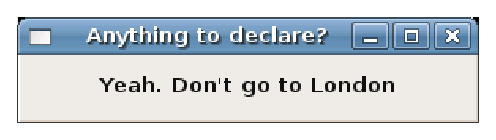
\includegraphics[scale=0.905]{images/london2.eps}
%% \end{center}

%% \verbatiminput{../examples/framework/hey/heyglade2.py}

%% Of course, it is often useful to subclass \code{BaseView} to be able to
%% customize the behavior that you want for that view. I recommend
%% changes that are to be done to the widgets at startup time (like
%% \function{set\_bold()} and \function{set\_size()} for a label) should be
%% performed in the class constructor, right after
%% \function{BaseView.\_\_init\_\_()}\footnote{Yes, in a way this is the
%% opposite of the procedure in \class{SlaveView} and \class{BaseView}. It
%% has to be this way because the parent constructor for \class{BaseView}
%% is who attaches the widgets to the view, whereas the constructors for the
%% other Views {\it expect} them to be already attached}. If you subclass,
%% you can skip passing \code{widgets} to the constructor by creating a class
%% variable with the same name.

%% An example of a subclassed \class{BaseView} using \code{widgets} as a
%% class variable follows (in the Kiwi tarball in
%% \file{Kiwi/examples/framework/hey/heyglade3.py}):

%% \verbatiminput{../examples/framework/hey/heyglade3.py}

\subsection{UI Composition}

The examples we have seen so far use a simple mapping: one View per
window. While simple applications will use this and nothing else,
wouldn't it be interesting to reuse parts of your interface just like
you reuse code when programming?

UI Composition allows you to create components of your application UI,
which in Kiwi are named {\bf slaves}, and attach them to other Views.
This allows you to embed widgets in any way you like. A slave is really
just another View (there {\it is} a class called SlaveView, which is for
interfaces without a toplevel window that do not use Glade, but any view
can be used as a slave) that happens to be attached to another view.

To implement this, Kiwi uses GTK+'s really cool ``reparenting'', a
property which allows a widget to be removed from one place in the
widget hierarchy and placed in the other (in Kiwi terms, a View's widget
is replaced by another View).

A view that will embed one or more slaves is called a Parent view
(though there is no class with that name; read on). There are two
important requirements for a Parent view:

\begin{enumerate}
\item {\bf The parent View must be a BaseView}. This allows us to
easily find a named widget and change it for a slave. No, there is no
ParentView class: it would be a useless, as there is nothing a
ParentView needs to do that a BaseView doesn't do already.
\item The {\bf parent View must contain a "placeholder" widget
identified by a name, inside an gtk.EventBox}, name being the Name: property
defined in the Widget tab in Glade. The part about EventBox may seem a
bit awkward, but it allows us to guarantee that the child packing of the
substituted widget will not change. If we were to swap simply a widget
for another, the first widget's container would loose the child packing
information (i.e., gtk.Box and gtk.Table's child attributes: expand, fill,
padding and span).
\end{enumerate}

I'll demonstrate by showing how a parent view is built in glade. Look at
\file{examples/Browser/news\_shell.glade}:

\begin{center}
\includegraphics[scale=0.905]{images/shell1.eps}
\end{center}

In \file{news.glade} I put together a simple dialog, and in the place where
I want the slave to be embedded, I have added an EventBox (with any
name) and a label (named \code{my\_placeholder}). We now write a
small SlaveView called \class{NewsView}:

\begin{verbatim}
from kiwi.ui.views import SlaveView
from kiwi.ui.objectlist import ObjectList, Column

class Item:
   def __init__(self, news, author):
       self.news, self.author = news, author

class NewsView(SlaveView):
    def __init__(self):
        news = ObjectList(Column("news", "News",),
                          Column("author", "Author"))
        for item in newsitems:
            news.append(item)
        SlaveView.__init__(self, toplevel=news)

# Some news articles borrowed from Pigdog Journal for our example
newsitems = [
  NewsItem("Smallpox Vaccinations for EVERYONE",
           "JRoyale"),
  NewsItem("Is that uranium in your pocket or are you just happy to see me?",
           "Baron Earl"),
]

\end{verbatim}

Now of course, this view can't display itself; it's a \code{SlaveView},
and it lacks a toplevel window. But that doesn't matter; we want to
attach it as a slave to a main View. We create \code{news}, an instance
of \class{NewsView}, and a \class{BaseView} instance called
\code{shell}, which will be our parent View. We then call the method
\code{attach\_slave()}, which does the actual reparenting; it takes as
arguments the name of the widget {\it to be replaced} and the view to be
attached. At this point, we run the parent view as we would normally:

\begin{verbatim}

from kiwi.ui.views import BaseView
news = NewsView()
shell = BaseView("news_shell", delete_handler=mainquit)
shell.attach_slave("my_placeholder", news)

news.show_all()
news.focus_toplevel() # explained next section, don't worry
shell.show_and_loop()
\end{verbatim}

In summary, I gather some random news, create a \class{NewsView}
instance, a \class{BaseView} instance (that will be the parent), call
the special function \code{attach\_slave()}, and that's it. (There is a
minor detail with widget focus that is discussed in the next section;
basically, the slave needs to be attached to the parent before trying to
focus its widgets).  The final result is shown below:

\begin{center}
\includegraphics[scale=0.905]{images/shell2.eps}
\end{center}

Note that all the examples up to now have been very simple and static:
there is no user interaction going on beyond closing the window (for
instance, the buttons in the previous example do nothing!). To be able
to handle events, we need to understand how the Controller classes (and
their derivates, the Delegates) work. The next section explains them in
detail.

\subsection{Controllers}
\label{callbacks}

In GTK+, all user events are interpreted by signals that are generated
by the widgets that are manipulated. This means obvious stuff like
button clicks and typing text into a \class{gtk.Entry}, but it also
includes less obvious events like the initial rendering of the widget
and moving the mouse over a widget. To a signal, we can attach a
function that is called when it is triggered, and this function is
usually called a {\bf signal handler}.

Many widgets have default handlers attached to their signals (these are
coded in the actual GTK+ source code); a default handler, for example,
is what makes the text that you type into an Entry actually display
inside its white box, and what makes the checkbutton depress and change
state when you click on it. However, there are many cases when you want
to do something special based on a certain signal occurring. A pushbutton
(\class{gtk.Button}) is a good example: it doesn't do anything by default
when clicked beyond depressing, so you practically always will want to
connect to its "clicked" signal. Developing a graphical application
involves selecting which signals you think are important in the
interface widgets, and attaching functions to them.

In Kiwi, we suggest grouping the relevant signal handlers for an
interface into a class. This means that instead of using a number of
independent functions, the signal handlers are really methods of
a class. This class is called the \class{Controller}. The
\class{Controller} is conceptually the part of the framework that
handles events that are generated in the UI; click a button, a
controller method is called.

Since the View holds the interface, it makes sense to attach a
controller to each view\footnote{Ancient versions of Kiwi had a
MultiView class, that held various subviews for portions of it, and
required one controller for each subview. The new SlaveView approach is
nicer, because it allows reusing the actual interface in a much more
flexible manner.}, and vice-versa; the Controller constructor takes a
View instance and ties itself to it. Since the controller needs to
define special methods, it should be subclassed in your code, and the
methods implemented.

The Kiwi Controller has a special feature: if you write your method
names using a certain syntax, it "discovers" what widget and signal you
want, and attaches the handler automatically for you. This works for any
type of View, even BaseViews, which means no more messing around with
\code{signal\_autoconnect()} and that pesky signal dialog in Glade. The
handler's method name should be written as follows:

\begin{enumerate}
\item Start the name with \code{on\_} or \code{after\_}. Use \code{on\_} to
connect before the default handler for that widget's signal; use
\code{after\_} to connect after it. It is more common to use
\code{on\_}\footnote{Hint: if you are connecting
to a \class{gtk.Entry}'s \code{insert\_text} signal and you want to use
\code{entry.get\_text()}, use \code{after\_entrywidget\_\_insert\_text}
--- the default signal handler is responsible for inserting the text
into the entry and you will need it to run before your handler.}.

\item Add the widget name: this is the name of the View's instance
variable for that widget.  If your view has a widget called
\code{quitbutton}, you would use "quitbutton".

\item Follow the widget name by two underscores (\code{\_\_}).

\item Finish the name by appending the signal name you want to capture.
For instance, if you wanted to handle that quitbutton's \code{clicked}
signal, you would use "clicked". The final method name would be
\code{on\_quitbutton\_\_clicked}.
\end{enumerate}

Note that the widget must be attached {\it directly} to the controller's
corresponding View; it can't be attached using this syntax to a slave of
that view, for instance (you'll have to call \code{connect()} directly
in that case).

Let's see a simple example to make
these concepts more concrete (included in the Kiwi tarball at
\file{Kiwi/examples/framework/faren/faren.py}):

\begin{center}
\includegraphics[scale=0.905]{images/faren.eps}
\end{center}

\verbatiminput{../examples/framework/faren/faren.py}

Let's have a look at the code. I define a Controller
\class{FarenControl} that inherits from \class{BaseController}, and
which defines two methods that are signal handlers - one for the
"clicked" event for the widget \code{quitbutton}, and another for the
"insert\_text" signal for \code{temperature}. I attach the view to the
controller, and tell the view to show itself and run the event loop. Not
much else is worth noting, apart from the fact that the signal handlers
receive the widget as the first parameter, and that the GTK+ text
widgets (gtk.Entry, gtk.Label, gtk.Text) usually take and return strings,
which makes us do conversion here and there.

Thus, the event loop now has two signal handlers that will be triggered
according to the user's interaction: one called when clicking the
quitbutton and one when inserting text into the entry. The user can type
numbers into the entry, and through
\code{after\_temperature\_\_insert\_text()}, the celsius and farenheit
labels are changed automatically. Clicking quit calls a special method
in the view, \code{hide\_and\_quit()}, that hides the window and quits
the event loop. Note that the widgets "celsius" and "farenheit" are
empty labels that appear right next to the labels that {\it are written}
"Celsius" and "Farenheit"; if you are confused look at the glade file
\citetitle[faren.glade]{faren.glade}.

\subsubsection{Default Widget Focus}

An important usability aspect of an application is having focus set by
default to the widget where it is most useful, so the user can start
working right away without having to tab his way through the window's
widgets. If you pay attention, when you first start the \file{faren.py}
example, the gtk.Entry for temperature starts with the cursor focus; I've
set the "Has focus" property to True for that widget {\it in Glade}.
\code{show*\_and\_loop()} checks your interface before running; if there
is an interactive widget attached to it, and none of the View's widgets
is focused, it prints a warning to standard error explaining the View
doesn't have an interactive widget focused:

    \begin{verbatim}
    Kiwi warning: no widget is focused in view
        <__main__.FarenView instance at 0x8335444>
    but you have an interactive widget in it:
        <Kiwi.Basic.Entry instance at 0x8774f14>
    \end{verbatim}

Setting the focused widget in Glade may seem unobvious; if so, you have
alternatives to set focus programatically:

\begin{itemize}
\item Call \code{grab\_focus()} on the specific widget you want to focus.
If you are using a subclassed View, I would recommend doing this at the
end of your View's constructor; otherwise, call it directly before
running \code{show\_and\_loop()}.
% If it's a bad idea, should we document it?
% \item Call \code{view.focus\_toplevel()}. This causes the toplevel
% widget to be focused, which is usually a {\bf bad} idea because it is
% normally a window or container.
\item Call \code{view.focus\_topmost()}. For most forms, it makes sense
to focus the form widget most to the top and left when starting up the
application; you can use this convenience function to accomplish that.
\end{itemize}

When using UI composition, remember that the slave view will lose its
focus state when the function \code{attach\_slave()} is run, so if you
wish to focus a widget that is part of the slave, you will need to do it
explicitly after that function call. If the widget to be focused is in
the parent view, you should have no problems (unless you are swapping
*that* particular widget for the slave, of course).

\subsubsection{Advanced Controllers}

While the previous section on Controllers offered a nice example with
the Faren application, it does present some issues. First, the interface
could use some extra niceness (deleting text from the entry does
nothing!). Second, the controller has to invoke methods on its view's
instance variables (\code{self.view.celsius.set\_text()} for example),
which is a sign of high coupling. One good way to solve these issues is
to provide a subclass of BaseView that does some extra setup and
provides an API for the Controller (\file{faren2.py}):

\verbatiminput{../examples/framework/faren/faren2.py}

This (much longer, sure, but with a nicer division) example shows us
using a separate View class, which presents an API for manipulating the
View interface widgets, consisting of the following methods:

\begin{itemize}
\item \code{get\_temp()}: Gets the temperature from the gtk.Entry in the
interface, and returns it. Returns None if the entry is empty.
\item \code{update\_temp()}: Updates the contents of the two labels that
represent the temperature (in farenheit and in celsius).
\item \code{clear\_temp()}: Clears the contents of the two labels that
represent the temperature.
\end{itemize}

The Controller also uses \code{changed} instead of \code{insert\_text},
so it supports both insertion and deletion.

This is basically what you need to know about the controller. While it
is useful in a number of applications, if your interface has a number of
widgets and rich interaction, you will notice that your View API will
start looking like a exact copy of the widget methods. This is highly
undesirable (as are accessor functions, for the same reason): it means
the Controller is tightly coupled to the View, which is not what we
want. And {\bf herein lies the main problem with the View/Controller
split}: if your interface is simple (as it is in our example), it's a
nice way to separate things; however, if your interface is complex and
has lots of widgets (I'd say a good rule of thumb is over 5 interactive
widgets) you will end up with a lot of low-level View/Controller message
passing.

(Another potential problem with the split is that neither the Controller
nor the View are very reusable, which defeats part of the goals of
modularity). The next section describes UI Delegates, which are
combinations of View and Controller that simplify things somewhat.

\subsection{UI Delegates}

The UI Delegate classes, located in the \module{kiwi.ui.delegates} module, use
multiple inheritance, being derived from both a View and a Controller.
This means they combine functionality from both into a single class: not
only does it specify the interface, it also handles the widget signals.
It's the "can't beat them, join them" solution to the V+C coupling
problem, and it's used in Swing, MFC and Bakery, a C++ framework for
GTK+.

The \class{Delegate} class is a combination of \class{BaseView} and
\class{BaseController}. You can use it to create your interface
programatically and then hook up handlers to it, just like you would do
to individual views and controllers. A very simple (yes, I too get bored
of hand-coding PyGTK widgets) example follows, found in the distribution
as \file{examples/framework/simple.py}:

\begin{center}
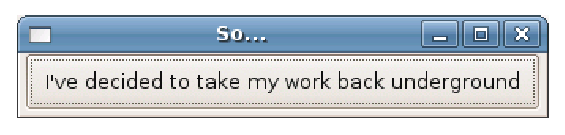
\includegraphics[scale=0.905]{images/simple2.eps}
\end{center}

\verbatiminput{../examples/framework/simple.py}

\begin{center}
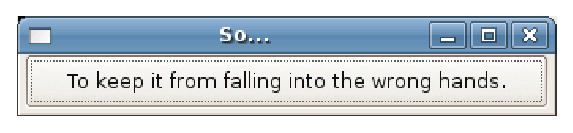
\includegraphics[scale=0.905]{images/simple3.eps}
\end{center}

As you can see, the Delegate was the only class we needed to inherit
from and instantiate. This makes the amount of infrastructure code go
down significantly, and most single-window applications (and individual
dialogs in multi-window applications) can be implemented with single
Delegate and GladeDelegate subclasses. As an example for using the
GladeDelegate, below is a third version of our temperature conversion
application, \file{examples/Faren/faren3.py}:

\verbatiminput{../examples/framework/faren/faren3.py}

As you can see, using the delegates makes a lot of sense in many cases:
the view and controller split isn't essential, and you can end up
with a lot less code with the same functionality at no reduced
maintainability or readability, which is what we are aiming for. For
larger applications, or apps where a lot of very unusual functionality
is required, it may still make sense to use separate Controllers and
Views, but for normal development, stick to delegates; they simplify
things.

Note that there is also a \class{SlaveDelegate}, which works like a
normal SlaveView with an attached Controller.

\subsection{UI Composition with Delegates (or Views and Controllers)}

As we saw before, it is possible to compose the interface for your
application using multiple views; this holds true whether the view has
an associated controller or not. I'm not going to provide an example
embedding views and controllers because it's not very enlightening; it
is easy to extend the original UI Composition example to use controller
associated to the views, and that example is much more interesting if
adapted to a ObjectList.

Since delegates inherit from views, it is also possible to compose
a delegate with multiple child delegates (and even mix and match them
with views). The requirement that the parent delegate be based on glade
is the same, too: you should subclass \class{GladeDelegate} for your
main window, though any kind of view can be attached to it.

The nice part about doing UI composition using delegates is that the
interface and interaction is well encapsulated in a single class, and if
you are careful when writing a child delegate, you can reuse that class
in as many places of your applications as you like.  I'm going to use
the ObjectList from the last example to build a (rather fake) news
browsing application in the next example:

\begin{center}
\includegraphics[scale=0.905]{images/news3.eps}
\end{center}

\verbatiminput{../examples/framework/news/news3.py}

Let's have a quick look at the code:

\begin{enumerate}
\item I create a list of instances and the columns specification; I then
define a class for the news shell, inheriting from
\class{GladeDelegate}.
\item In the constructor I show off some cosmetic features of Kiwi (the
"header" widget is an eventbox, in which the label is a child; look at
the glade file for more details).
\item I create and attach the slave, storing a reference to it in the
instance variable "slave", and set focus up.
\item I define handlers for the buttons, and the simple handler
\code{row\_selected()} for the \code{select\_row} signal, which will be
called when a row is selected.
\item I create and run the \class{Shell}, which renders the interface.
When the interface closes, I catch the return value \code{retval} and
use it as input to run a browser for the selected news item (okay, so
the app is not really a browser, I lied).
\end{enumerate}

This example shows a lot of the power of Kiwi; in a few lines, and with
a little work in Glade, we have a working application that looks decent,
behaves well and isn't hard to maintain. The next section will go on
describing Proxies, which are high-level Views that represent an
instance or part of it.

\subsection{Proxies and Models}

This section describes a set of important high-level classes that Kiwi
offers, the Proxies. Proxies are special types of Delegates that attach
themselves to instances, and allow changes performed in the UI to
reflect automatically in the instance. This section does an introduction
to the concepts involved and then moves on to implementation details.

\subsubsection{Domain Objects (or Models)}

Doing Object Oriented (OO) implementation implies the system you are
creating revolves around objects; in the case of Python applications, we
use the word `instances'. OO applications call the instances that
represent your problem's logical entities
\citetitle[http://c2.com/cgi/wiki?DomainObject]{'domain objects'}. In a
mail application, for instance, you might have Person and Message domain
objects; in a sales application you could have Product and Sale.

Picking up from our last example, you could say \class{NewsItem}
represented a class of domain objects, since its instances held data (or
`state') that represented a logical container relevant to the task we
had at hand, browsing news.  This example was very simple, and there was
no mechanism coded into the \class{NewsItem} class, but the concept is
the same.

One very common problem when coding a new UI to manipulate the
information in a domain object -- at the fundamental level, in an
instance -- is the amount of code that needs to be done to alter the
state of the instance. If you have a small form, with few controls in
it, it's merely a bother; if you have a complex form, with many controls
and lots of interaction, it can be a nightmare of accessors and message
passing. Each widget must have the appropriate signals connected, and
the handlers must either manipulate the instance directly, or call
accessors repeatedly. Changing the UI involves more coding and
complication.

So, in summary:

\begin{itemize}
\item I use the terms {\bf object, model\footnote{A note on naming: in
MVC, one third of the triad is called Model, which (I believe) is short
for Application Model. In theory, the Application Model represents the
real-world behavior of your application, just like the domain object;
synonyms, basically. Some authors, however, defend that the Application
Model and the domain object should be separate entities. I don't think
this is necessarily true.  From my experience, in most cases the two are
functionally equivalent (and separating them showed me that I ended up
doing was proxying calls from one to the other).} and instance}
interchangeably to refer to a {\bf domain object}.
\item The problem at hand is propagating changes from the UI to the
domain objects attached to them.

This is the task Proxies attempt to simplify.
\end{itemize}

\subsubsection{Using Proxies}

As stated before, Proxies attempt to reduce the "glue" code between UI
and domain object.  They work by attaching themselves to the model,
detecting the widgets in the interface, attaching the correct signals to
these widgets, and providing handlers that manipulate the attached model
in a standard way.  The updating mechanism works by associating selected
widgets in the Proxy to attributes in the model; if the model offers
accessors to these attributes, they will be called, and otherwise direct
manipulation of the model attributes is performed. {\bf This association
is done by name}: the names of the widgets determine the name of the
accessors or attributes that will be used in the model.

There are two types of Proxy classes: \class{Proxy} and
\class{ProxyDelegate}. Their constructors are similar to their Delegate
counterparts, the main difference being a new parameter, \code{model},
which specifies the instance that we should attach this proxy to.
%XXX: Explain about add_widgets()
%The Proxy's \code{widgets} list uses an extended syntax: the
%widget names that are to be associated to attributes should be prefixed
%by a single colon character ({\bf :}).  This prefixing should be done
%*only* in the widgets list - the name in the glade file, the model and
%the callback syntax should not include it.

%For the first example, let's attach a proxy to an interface specified
%in glade (\file{examples/framework/newsform/newsform.py}):

%% \begin{center}
%% \includegraphics[scale=0.626]{images/newsform.eps}
%% \end{center}

\verbatiminput{../examples/framework/newsform/newsform.py}

Let's look at this simple example. First, I define a model class which
is really just a shell class, with no methods or attributes:
\class{NewsItem}. We create an instance of this class, define the
widgets list (that will correspond to the model attributes), and create
a new proxy, specifying \code{item} in the constructor.

After running the Proxy, there is a print call that outputs the
attributes from the \code{item} instance. Note that these attributes
were not defined initially in the model: this is not a problem; the
proxy will set them to sensible values on startup. If you run the
program, enter data in the entries, and close the window, you will also
see that the values printed out at the end correspond to the values
typed in.

Note that we don't need to define any handlers for the Proxy's widgets.
This is the Proxy's "magic" - it defines internal handlers that take
care of updating the attached model automatically. As we insert and
delete text from the entries, the model is being transparently updated
to reflect the new value in the interface. In this way, the interface's
state is synchronized with the model's state.

\subsubsection{Propagating changes from Model to Proxy}

In our previous example, our model was defined as an instance of a
simple Python class. If we use the complete framework, by having our
model classes inherit from \class{FrameWork.Model}, we also get reverse
notifications from Model to Proxy: when the model is altered, the change
propagates to the proxy interface attached to it.

To demonstrate, we can extend the example above to add a "reset" button
to trigger a change of the model; we will subclass ProxyDelegate (which is
also a Delegate, as stated before, and thus supports the special handler
syntax \code{on\_*()}) to define a handler for clicking on the reset
button (\file{examples/framework/newsform/newsform2.py}):

%% \begin{center}
%% \includegraphics[scale=0.626]{images/newsform2.eps}
%% \end{center}

%% \verbatiminput{../examples/framework/newsform/newsform2.py}

If we look at the handler for reset, \code{on\_reset\_\_clicked()}, we
can see it alters the model directly. These changes reflect
automatically in the interface by means of an update mechanism present
in \class{FrameWork.Model}. This holds true no matter what function
triggers the change in the model: it is not limited to callbacks defined
in Proxy itself; any handler that alters the model will trigger the
model's update mechanism.

In summary: if you need to alter your model independently of the
interface, have your model inherit from FrameWork.Model and enjoy
automatic UI updating.

In all the examples we have shown up to now, you may notice that the
proxy manipulates the model's instance variables directly. There are
times where this is not desirable, and the next section explains how to
customize the proxy and model's behavior.

\subsubsection{Customizing Proxies and Models}

From our example, proxy and instance appear to be completely coupled -
even the names of the components and attributes are tied. This is a
precise interpretation of the situation, but in my opinion, this
coupling is not only unavoidable, it is the essence of UI architecture.
Treating the interface as a completely separate entity from the object
it manipulates is, honestly, a bad idea, because {\bf the interface is a
representation of the object}, and as such, essentially coupled to it.
Would it make sense to remove the \code{url} attribute from the model
and {\it not} remove it from the interface in question?

Because the UI is really a representation, however, there are times
where the contents of the widget and its attached proxy attribute must
differ in some way. Often, it is a matter of cardinality: more than one
widget defines a single proxy attribute, or vice-versa; at other times,
the data format in the widget does not match the format in the model
(think of dates, represented by strings in the interface, but stored as
DateTime objects in the object)\footnote{ Apart from these reasons, some
people insist that it is bad or wrong to manipulate the instance
directly, and that accessors should always be used.}. The Kiwi Proxy was
designed to cater to these different requirements, using accessor
functions when available.

Accessors provide an easy way to translate the model value to the
interface value: a pair of \code{get\_*()} and \code{set\_*()} functions
implemented in the model that perform internal manipulation of its
variables, removing the need to directly manipulate the instance
variable. You can define accessors for as few or as many model
attributes you want.

To make the process clearer, it is worth discussing how the model and
the UI are updated. The heuristics for updating a model are:

\begin{enumerate}
\item If a change happens in the Proxy's widget \code{X}, it looks at
the model attached to it.
\item If the model offers a \code{set\_X()} method, it is called, with
the new value as its only parameter.
\item If not, it manipulates the model directly by using
\code{setattr()}, which is the equivalent of \code{model.X = value}. If
\code{Proxies.set\_attr\_warnings(True)} has been called, a warning like
the following will be printed:

    \begin{verbatim}
    Kiwi warning: could not find method set_title in model
    <__main__.NewsItem instance at 0x82011ac>, using setattr()
    \end{verbatim}

\item The model is updated (If multiple proxies are attached to the
model, special things happen, additionally, as you will see in section
\ref{multipleproxies}).
\end{enumerate}

The heuristics for updating the interface widget are:

\begin{enumerate}
\item On startup, the proxy queries the model for the value for
attribute \code{X}.
\item It tries first using an accessor method \code{get\_X()}
(which should return a single value). If the accessor does not exist, it
will attempt to access the model's variable directly (using
\code{getattr()}). As with \code{setattr()} above, a warning will be
printed if attribute warnings are enabled.
\item The interface is updated with this initial value, and normal
event processing begins.
\item If a model's state for \code{X} is altered (\code{item.X =
"foo"}), a notification is sent to the proxy, with the attribute that
was altered. If a callback calls \code{self.update("X")}, a notification
is sent to the proxy, with the attribute that was altered.
\item The proxy receives the notification; it gets the value of \code{X}
from the model using the same method as in step 2, and updates the
widget contents accordingly.
\end{enumerate}

Summarizing: if you would like to customize the connection between model
and proxy for an attribute, implement accessor functions
(\code{get\_foo()} and \code{set\_foo()}) for it. If you would like to
verify that no direct instance manipulations are happening, use the
module function \code{set\_attr\_warnings()} and check the output
printed to the console's standard error.

Let's extend our previous example to provide an accessor and explain how
things work out (\file{newsform3.py}).

\begin{verbatim}
    class NewsItem(FrameWork.Model):
        """An instance representing an item of news.
           Attributes: title, author, url"""
        def set_url(self, url):
            """sets the url, prefixing "http://" if missing"""
            http = "http://"
            if len(url) > len(http) and string.find(url, http) != 0:
                url = http + url
            self.url = url
\end{verbatim}

In this example, we provide an accessor for setting the url (a "setter")
prefixed by "http://". The accessor is called when the entry's text
changes (for each character inserted or deleted), which is why I have to
check for the length of the url typed in. Note that I don't provide a
\code{get\_url()} method (a "getter"), which means the raw url would be
loaded from the instance into the interface. In this specific case, this
is not an issue, because data is only loaded from the instance at
instantiation time and when the model attribute is changed. However, for
most cases both setter and getter need to convert to and from the model
format.

\subsubsection{Using Signal Handlers in Proxies}

Proxies implement their behavior by using GTK+ signals extensively, but
this mechanism is implemented inside the Proxy and most of it happens
automatically, without user-visible effects beyond updating of the model
and the interface. However, many times an application needs custom
behavior beyond the simple model updating; for this, user-defined
handlers can be used normally.

Proxies inherit from the Delegate classes, and they can define signal
handlers in the same way as normal Delegates (and Controllers), by using
the special syntax as defined in section \ref{callbacks}. However, there
is a special detail that should be understood when using custom
callbacks:

\begin{quotation}
{\bf The Proxy's internal callbacks are executed first}.
\end{quotation}

This means that, when your \code{on\_*()} or \code{after\_*()} handler
runs, the Proxy has already updated the model. In practice, this is a
{\it good} thing, since you usually want to work with the current
contents of the widget, not the contents it used to have. Of course,
signal handlers in the Proxy that are not associated to widgets attached
to model attributes (in other words, widgets not prefixed by a colon
(:) in the widgets list) do not present this issue (as there is no Proxy
signal handler for them anyway).

One common task of using signal handlers is to trigger updates in some
other part of interface. For instance, you might have a radiobutton that
makes a certain part of the interface sensitive when toggled. Or an
entry that needs to update a label that represents a calculated field in
the interface. You can define handlers normally, and you can take
advantage of the special Proxy method \code{update({\it
attribute\_name})}, which notifies the Proxy that it should refresh the
interface representation of that attribute.

%As an example, I will include here a final version of the Faren application
%that uses a Proxy (\file{../examples/framework/faren/faren4.py}):

%% \verbatiminput{../examples/framework/faren/faren4.py}

A step-by-step analysis of this example:

\begin{itemize}
\item We define a class for our domain object, \class{Temperature}. This
class offers accessors for two "fake" attributes - they don't exist
permanently in the instance, but instead are calculated through
accessors. Note that we {\it must} initialize any values that we use in
the accessors, as they will be called upon startup; temperature will not
have been set through the interface at that point yet.

\item The accessors return an empty string if temperature is an empty
string, and calculate the values otherwise. This agrees with the
behaviour defined for this application before: an empty temperature
should render no output for farenheit or celsius.

\item We create a proxy class for our application.  We first set a
conversion format for \code{farenheit} and \code{celsius} so it will
print out the float values they return correctly. \code{set\_format()}
is discussed further in section \ref{formats}.

\item We then initialize the parent class, using the same glade file as
the other Faren examples. We do basic cosmetic updates, and then define
two handlers.

\item The first handler is simply for quit, and doesn't do anything
special. The second handler, however, is triggered whenever the
temperature is changed, and it uses the special \code{update()} method
to notify the proxy that both \code{farenheit} and \code{celsius} were
updated.

\end{itemize}

Upon running the example you will see that it works as expected;
the \code{update()} messages in fact make the labels render the correct
values, and the accessors return empty strings when they should.

There is an additional hook you can use in your Proxy classes to make
updating easier. If you define a method called \code{proxy\_updated()},
this method will be called {\it each} time a proxy-managed widget is
manipulated by the user. This allows you to easily perform updating of
calculated text indicators, for instance.

There is a set of more complex examples that demonstrate the use of
custom handlers in the package, under the directory
\file{examples/Diary}, which are recommended as further reference.

\subsubsection{Widget support in Proxies}

The Proxies provide a quite complex mechanism to handle updates in most
of the widgets normally used in "forms". There is a reason for
supporting these widgets: they are easily mapped to model attributes.
This doesn't mean that you can't use other widgets in your Proxy
interface, but there is no automatic update mechanism for it, and you
will have to use your own handlers for them.

This is a reasonable property -- it would be difficult to map what
exactly the state of a gtk.Curve means to the model, for instance -- and
the Proxy can be extended in the future to support other widgets (write
me if you are interested in contributing). What follows is a list of
widget types supported, details on the use of them, and details about
setting custom handlers if you need them.

\begin{itemize}
\item {\bf gtk.Entry}: the single-line entry box in gtk. Updates the
model on insertion or deletion of every character, which means you
should make sure your accessors take this into account, if you use
accessors (as opposed to \code{setattr()}). For instance, if you type in
"Foobar" into the box, the accessor for that model attribute will be
called 6 times.

{\bf Custom handlers}: The best signal for hooking a user handler to a
gtk.Entry is "changed", preferably by using \code{after\_{\it
entryname}\_\_changed()}; it will be called immediately after the entry
has text inserted or deleted. You can use the individual "insert\_text"
or "delete\_text" signals if you want to capture one of those specific
events.

\item {\bf gtk.Label}: a read-only widget that displays text. It is
useful for displaying model attributes, but it doesn't generate signals
my itself. Use \code{update()} in other widget's custom handlers to
notify the Proxy a calculated label's value has changed.

{\bf Custom handlers}: The gtk.Label doesn't generate signals.

\item {\bf gtk.OptionMenu (OM)}: the menuitem or listbox widget,
containing a list of items. The GTK+ OM has a very evil API by default,
but using the Proxy makes it much simpler; basically, the OM's choice
reflects directly in the model, without extra effort. The OM items can
be created in Glade or straight PyGTK commands; in this case the model
attribute will be set to the text in the label selected. To select an
item, set the model value to the string of text. The model is updated
each time an item is selected in the OM.

However, this is a very limited way of using the OM, and the recommended
way to build your menu is to use Kiwi's \code{OptionMenu.prefill()}
call, which allows you to specify a data value for each item, along with
an extra callback to be called when the an item in the OM is selected.
This way, the model's attribute can be set to any value per item; for
instance, an integer value, or an instance associated with one
particular menuitem.

If you use \code{OM.prefill()}, each item is associated to a data value,
and this value is sent to the model when the item is selected. To select
an item from the model, just set the attribute to the data value, and
the optionmenu updates itself automatically. Set the model attribute to
the data value, and the interface updates automatically. Check the API
for OM for more details.

{\bf Custom handlers}: as stated above, use \code{prefill()}'s
\code{callback} parameter to specify a handler for the OptionMenu.
There is no signal you can connect to directly in GTK+ 1.2.

\item {\bf gtk.RadioButton}: Handling the radiobutton is slightly more
complicated, because there are in reality groups of radiobuttons that
bind to a single attribute. In other words, the multiple radiobutton
widgets are connected to a single attribute, which assumes a different
value depending on which button is toggled.

To perform this grouping\footnote{Alas, we can't use radiobutton's
\code{group()} method to discover groups automatically because it is yet
to be wrapped in PyGTK.} the Proxy offers a special method called
\code{group\_radiobuttons()}. This method accepts \code{name} and set of
tuples as a parameter, each tuple being in the format \code{({\it
widget\_name}, {\it widget\_value})}. \code{name} indicates the model
attribute it is to be bound to, \code{widget\_name} is a string strings
with the name (like used in the widgets list) of the individual
radiobutton to be grouped. Once grouped, these radiobuttons are treated
by the Proxy as a single widget attached to the model attribute, and the
model attribute or accessor will receive the \code{widget\_value}
associated with the button selected. Setting the model value follows the
same rule as for OM.

{\bf Custom handlers}: use the "clicked" signal, connecting after it
(see gtk.Entry above for an \code{after\_*()} example), and check the
state of the widget if you need to check if it was selected or
de-selected (use \code{widget['active']} to check the state in your
callback).

\item {\bf gtk.CheckButton} and {\bf gtk.ToggleButton}: the two-state
button widgets allow values to be set to True and False.
The value is updated every time the button's state changes.

{\bf Custom handlers}: use the "clicked" signal, in the same manner as
for gtk.RadioButton.

\item {\bf gtk.SpinButton}, {\bf gtk.ComboBox} and {\bf gtk.TextView}:
similarly to the gtk.Entry, these widgets are updated every time a
single character is changed in the editable space (yes, the SpinButton
contains an entry). There is no signal that can easily catch when a
gtk.ComboBox list item was selected, which is why we have to handle
things this was for it. In practice, it should work as expected unless
you rely on your accessor being called a specific number of times for
each change, which you shouldn't.

{\bf Custom handlers}: gtk.SpinButton and gtk.Text are good candidates for
the "changed" signal; use the same rules as for gtk.Entry. For gtk.Combo,
things are not so easy, because there is no signal it offers you can
catch\footnote{A lively discussion could ensue about gtk.Combo and the
lack of a signal that indicates an option was selected in its list, but
I deliberately choose to avoid it!}, and the fact that it holds two
subobjects, a gtk.Entry and a gtk.Button, means that you are forced to use
\code{connect()} on either of these to get the effect you desire. In
practice, the following works for me (taking into account the fact that
the handler will be called multiple times):

    \begin{verbatim}
    widget = [":combo", ...]
    def __init__(self, *args):
        # [... in constructor ...]
        entry = combo.entry
        entry.connect("changed", on_combo_entry__changed)

    def on_combo_entry__changed(self, entry, *args):
        # [...]
    \end{verbatim}

\end{itemize}

The code in \file{tests/test\_Proxy.py} offers a sample of using all the
supported widgets in the same interface, and is highly recommended for
study; it is however a bit too long to include in this text.

\subsubsection{Models}

The \module{kiwi.model} module \class{Model} classes. As discussed
before, the \class{Model} class provides a mechanism for updating the
user interface based on changed performed in the model instance.

This is a powerful mechanism that allows you to guarantee that the
interface is always up-to-date with relation to an instance; it should
be used with care, however, because the update semantics are not trivial
to understand -- just imagine having custom callbacks that alter the
same attribute as the proxy callback and you will understand why it is
easy to get in recursive loops. This tip I can offer you, therefore:
avoid altering the model in custom callbacks, and only do it in special
situations.

You can also attach multiple proxies to the same model and have them
update automatically; the next section will discuss this further. Before
passing on to that, however, I need to describe a special \class{Model}
called \class{PickledModel}. To demonstrate by example, I will revisit
the first example we saw in this text, the Person editor from section
\ref{person}. Let's see the code again:

\verbatiminput{../examples/framework/person/person.py}

Looking at the code, you might notice three special issues:

\begin{enumerate}
\item The class our model inherits from is \class{FrameWork.PickledModel}.
\item We actually get our model instance by making a call to
\code{Person.unpickle()}, passing the class \class{Person} as
an argument.
\item We call \code{person.save()} at the end of the program.
\end{enumerate}

\class{PickledModel} offers a very cheap way to offer persistence for
your model instances. If you are familiar with the ZODB, think of
\class{PickledModel} as a cheapo implementation that allows you to save
and restore an instance. To use it:

\begin{enumerate}
\item Have your model class inherit from PickledModel.

\item Use the \code{PickledModel.unpickle} which is a class method on 
your model. it takes a filename as the optional second parameter (if omitted, 
it uses the name of the class, with an extension of ".pickle"). 
The method will try and load the model state from a pickle file, 
and if it doesn't exist, will create a new model and return it to you. 
If the pickle file is damaged, it will save it with the extension ".err" 
(avoiding it being erased by an unwitting \code{save()} call).

\item Use the \code{save()} method to save the pickle when you are
ready. You may specify a filename to it; otherwise, it uses the default
filename specified through the \code{set\_filename()} method. Note that
\code{PickledModel.unpickle} makes the filename it tried to used the 
default by calling \code{set\_filename()} internally.
\end{enumerate}

The \file{diary3.py} example in \code{examples/diary/} uses pickling in a
more involved manner and is recommended as a reference.

\subsubsection{Multiple Proxies}
\label{multipleproxies}

One feature of the \class{Model} class is that it allows multiple
proxies to be attached to the same model, performing automatic
notification to all of them. Internally, when a proxy attaches itself to
a model, it lets the model know what attributes it is interested in;
later, when that attribute changes, the model lets the proxy know.  The
syntax for using multiple proxies is straightforward; simply create the
proxies and attach the same model to them. A small example
(\file{NewsForm/newsform4.py}) follows:

%% \begin{center}
%% \includegraphics[scale=0.626]{images/newsform4.eps}
%% \end{center}

%% \verbatiminput{../examples/NewsForm/newsform4.py}

This example shows some of the power of multiple proxies; as you edit
the title you can see the label update immediately. If you look at the
lines at the bottom, two proxies are attached to \code{item} - a
\class{NewsProxy} instance, and a \class{NewsLabels} instance, which has
labels that display the current contents of the model.

This feature can be used in many different ways, and if you create small
proxies (that represent a part of the model, instead of the whole model)
and embed them in other interfaces you can end up with very dynamic
representations of your data. However, it should be noted that there are
a few gotchas that you can run into when using multiple Proxies:

\begin{itemize}
\item Trying to edit the same value in two proxies. This is actually
possible, but it is a bad idea, both UI-wise and implementation-wise. If
you are using multiple proxies for a single model, have only one be
editable and the others read-only (displaying information using labels,
for instance). See in our example how the use of labels only in
\class{NewsLabels} fits nicely into this rule.

\item Attaching two proxies to the same model and forgetting about it.
This can be quite misleading and hard to debug if you have a large
application. If you have many proxies for the same class, and they are
instantiated and run simultaneously, it may be tricky to notice that the
model sends messages to update both when it changes. Thankfully, it is
not common to have two windows with the same data loaded in the
application. This is related to the "Undo" problem discussed further in
section \ref{undo}.
\end{itemize}

\subsubsection{Other Proxy features}

Proxies are complex and featureful beasts; this section discusses some
additional details on them.

\paragraph{Types}

GTK+ treats most of the information in the interface as strings - its
API usually takes data as strings, and it returns strings. However, this
is a bit of a problem when dealing with an associated model, since the
model may very well use integer, float or any other types internally.

For numeric types, Proxies have special support. On startup, the Proxy
will look at the attached model and try and detect what attributes are
numeric, by looking at their current values. Of course, if there is no
value in the model, or it is a string, it will be assumed to be a
string; however, if it is a number (float or integer) it will be
remembered, and the Proxy will convert it from the GTK's internal string
to a numeric type before sending it to the model. Note that this
conversion is rather dumb and if invalid characters are used, exceptions
will be raised (that's about it, though; the mainloop allows the
application to go on running); use a validated Entry\footnote{To be
released in the next version of Kiwi, but some examples have been posted
to pygtk-list} to avoid this problem.

For other types, you must convert from strings using getter and setter
methods. If dealing with numeric types, you can also manually convert in
the \code{set\_*()} method and avoid any risks.

\paragraph{Formats}
\label{formats}

To avoid needing to provide accessors to deal with simple format
conversions, Proxies provide a way to set Python format strings that
will be applied to the attribute value when it is being applied to the
widget. The syntax is: \code{proxy.set\_format({\it attribute name},
{\it format string})} -- the name is a string with the name of the
attribute. You can pass a list of strings, optionally, to apply the same
format string to multiple attributes.

Note that this does {\it not} apply to the data that is set {\it to} the
model from the interface; it will be send without any conversion. Think
of it as a simple, one-way filter for data sent from the model to the
interface.

\paragraph{"Instant-apply" and Undo}
\label{undo}

The proxy can present something of a hazard for complex applications if
its "instant-apply" model is not understood completely. Instant-apply
means that, at any time, the UI and the model have the same state. If
you pop up a dialog with a Proxy, and you alter the model, even before
clicking "OK" the value in the model will have changed.

This may cause two classes of problems. The first is undoing the changes
performed upon the model during manipulation of the Proxy (think "cancel
button" if you are having a hard time imagining why). Solutions:

\begin{itemize}
\item One solution would be to store the initial state of the instance -
\module{pickle} can probably be used for implementing this. If Undo is
necessary, just reset the state of the model to the saved state. I have
not yet tested this, but I think it would work.

\item If you are using Zope.com's {\it excellent} database
\citetitle[http://www.amk.ca/zodb/]{ZODB}, you already have undo and
rollback mechanisms in your persistent objects, and all you need to do
is call the appropriate method and your model state is back to the
previous state.

\item Kiwi may at some point offer undo functionality, which would allow
one to undo selectively changes done to the model in the Proxy. At the
moment, this is just an idea, but I imagine it would not be hard to
implement.
\end{itemize}

The second problem is using the model in another part of the application
simultaneously (think "I am editing a price at the same time she is
selling the product"). This problem can be aggravated when using
multiple proxies attached to the same model. Solutions:

\begin{itemize}
\item You can offer a copy of your instance as the actual proxy
instance, and upon finishing editing using the proxy (or upon
"committing" the changes) you can transfer the state from the copy to
the real instance. This way, the application continues using the real
instance normally, and the proxy uses the copy without risking hard to
the application itself.

\item The Proxy could implement this solution internally, too; an idea
would be a sort of GhostProxy, which had a \code{commit()} method which
copied state automatically from the "ghost" to the real model.
\end{itemize}

(Yes, this part needs more research. I'll be looking into it.)

\paragraph{Proxy startup values}

When starting up a Proxy, the model attributes to be attached to the
Proxy are analyzed and the initial state of the Proxy interface is set.
The process by which this is performed is rather involved, and for the
sake of completeness (debugging these things can be a bit tiresome), is
listed here:

\begin{itemize}
\item If the model's attribute value is {\bf unset}, and there is no
accessor, the default value in the interface (specified in Glade or GTK
previously to initializing the Proxy) is used {\it and is set to the
model attribute}.
\item If the instance variable is set but is \code{None}, the following
defaults are used for each widget:
    \begin{itemize}
    \item {\bf gtk.Entry, gtk.Label, gtk.Combo, gtk.Text, gtk.SpinButton}: an
    empty string is set to the model, and a blank widget is presented.
    \item {\bf gtk.RadioButton}: The button set in Glade or GTK as
    initially on is selected, and if none is selected, the button that
    is most to the top and left of the Proxy interface is selected. The
    value associated with the radiobutton is set to the model attribute.
    \item {\bf gtk.OptionMenu}: the first item in the menu is selected, and
    its value is set to the model attribute.
    \item {\bf gtk.ToggleButton and gtk.CheckButton}: the widgets are set
    to unselected, and the model attribute is set to 0 (zero).
    \end{itemize}
\end{itemize}

\section{Widgets}

Besides the Framework, Kiwi also provides a set of widgets extending
existing widgets in GTK+.

% \subsection{Entries}

% \subsubsection{Masks}

% \subsubsection{Validation}

% \subsubsection{KiwiEntry}

% \subsubsection{ComboEntry}

% \subsubsection{DateEntry}

\subsection{ObjectList}

There is a special gtk.TreeView wrapper that accepts a list of columns,
each row of the list representing an instance. This is the first
high-level class of the framework being described; high-level in the
sense that it goes beyond simply organizing the UI and handler methods,
offering functionality directed towards object-oriented development in
Python.

The ObjectList was designed for the very common task of presenting a
list of instance data in a gtk.TreeView. Elaborating an example: lets say we
have a set of \class{Person} instances stored somewhere, each of these
instances possessing the attributes \code{name}, \code{address} and
\code{telephone}. A common problem is displaying a gtk.TreeView with this data
and performing an action when a person is selected. This is exactly the
use case which ObjectList supports.

Before showing an example, it's important to explain how the
ObjectList's constructor works, since it is rather special.

    \begin{verbatim}
    class ObjectList:
        def __init__(self, columns, instance_list=None,
                     mode=gtk.SELECTION\_BROWSE)
    \end{verbatim}

The ObjectList takes a \code{columns} parameter, and understanding it
is essential to using it correctly. \code{columns} should be a list of
\class{Column} instances, each of these instances representing a column
in the list (and therefore, an attribute in the instance). Let's have a
look at the constructor for \class{Column}:

    \begin{verbatim}
    class Column:
        __init__(self, attribute, title=None, data_type=True,
                 **kwargs)
    \end{verbatim}

Each Column instance determines the properties of the ObjectList's column;
most important of these is \code{attribute}, which specifies the name of
the instance attribute the column should hold. Note that all of these
arguments but \code{attribute} are optional and can be safely be left
out. To create a ObjectList for our example above, with columns for "name",
"address" and "telephone", we could have something like:

    \begin{verbatim}
    my_columns = [
        Column("name", sorted=True),
        Column("address"),
        Column("telephone", title="Phone")
    ]

    objects = ObjectList(my_columns)
    \end{verbatim}

This section of code would create a new ObjectList with 3 columns,
being sorted by the first one, and using "Name", "Address" and "Phone"
as column titles. See the API reference for \class{ObjectList} and
\class{Column} to find out all the details on them; there are many
features, including sort ordering, tooltips, format strings and more.

Note that you can produce a complete \code{column} specification by
running the delegate once with a simple set of columns, manipulating
them in runtime (changing sort order and widths, hiding columns) and and
then calling \code{dump\_columns()} on the delegate; this method creates
a list of \class{Column} instances corresponding to the current state of
the ObjectList. This list can be reused in the ObjectList constructor,
making it easy to save and restore the ObjectList's state even between runs.

The \code{instance\_list} parameter should provide a list of instances
to be inserted into the clist, and the handler is an optional callback
that will be run when items are selected in the clist. The instances in
the list {\bf must} offer either an accessor to the attribute specified
-- the accessor name must be in the format \code{get\_{\it
attribute\_name}}() -- or an attribute with the name specified (the
delegate will do a \code{getattr()} for it). Note that you can
instantiate a \class{ObjectList} without a list and add it later by
calling \code{new\_list({\it instance\_list})}.

To exemplify the ObjectList, I'm going to build upon the News Browser
example we saw a while back. I'm going to need to change the news data
structures from tuples to instances, and create a ObjectList for
it (see \code{news/news2.py}):

\verbatiminput{../examples/framework/news/news2.py}

Wow! Assuming you have data in the correct format, in some 25 lines you
defined the data for your applications, and in about 5 lines you
set up and created the ObjectList.  This example, though, doesn't do
anything (try running it - it doesn't even flash a window open, which is
what normally happens if you create a window but don't run the mainloop)
because {\bf a SlaveView doesn't have a toplevel window associated to
it}. To be able to use the ObjectList, we need to perform UI
composition: attach it to a parent view. I'll show for now a screenshot
of the generated widget inside a single window just so you know how it
looks:

\begin{center}
\includegraphics[scale=0.88]{images/news2.eps}
\end{center}

If you look at this image, you might notice some important details:
\begin{enumerate}
\item There is a little arrow in the right corner of the Title column.
What is that? A sort indicator! The titles in the first column are
sorted ascending. The ObjectList is set up so that you can order it's columns
by clicking on the headers, and it even sorts numeric data properly. By
default the sorted column is the left-most one, but you can change that
by using the columns spec.

\item There is a popup menu in the right corner of the image. What is
it? It's a list of the columns, allowing you to select which column is
displayed and which is hidden. As you can see, the URL column is hidden
(remember the False we passed in the \code{my\_columns} list?) and
Title and Author are displayed.

Note that both features are built in to the Kiwi ObjectList, one of the
enhanced widgets we provide.
\item (The gtk.TreeView has no window border around it. That's because I had to
do some magic to get this screenshot to display correctly. Don't worry
about it.)
\end{enumerate}


\section{References}

What follows in this section are references to FrameWorks and MVC that I
have collected from the Web and commented about. Each reference has a
bit of rambling I did when trying to understand what the papers meant,
and as such are biased towards what I think is right.

{\bf Mukul Sood}:
\citetitle[http://www.ddj.com/documents/s=916/ddj9809m/9809m.htm]
    {What is Swing}

\begin{quotation}

    Made some interesting points about the JTable. The JTable is a form
    generator based on a model. You specify if the property is editable,
    if it's a boolean, etc, and the JTable knows how to render it - as
    an editbox or as a label, as a checkbox, etc. You can register
    handlers for each of the types (editbox or a custom edit widget for
    editable properties, for instance).

    I wonder how it handles OptionMenu, but it does seem to. :)

    In Kiwi part of this is taken care of by CList, but there
    are some differences. First, the CList widget is rather limited, so
    you can't have checkboxes or editables in it (which is what the
    ListView *does* allow in GTK2) - it just takes the model and

    There is a major difference in how Swing handles the Model. In Kiwi
    the Model is the domain object proper, because the UI is specified
    independently. In Swing (and in the GTK2 ListModel, too), there is a
    Model that the UI is based upon, and your domain Model. In a sense,
    the Glade file is what makes us avoid specifying the UI Model in
    Kiwi, since the UI elements are already taken care of.

    In the example in this article, there is an AppMain class that is
    what is created when the app runs. The AppMain creates an
    AppController which takes care of initializing the Model and View.
    The View, however, holds the JTable, which in itself is a Delegate!
    This means part of the signals are treated internally by the JTable
    delegate, and a part by the AppController ("The mouse handler is
    implemented in AppController"). I don't know if I like this too
    much.

\end{quotation}

{\bf Sachin Deshpande}:
\citetitle[http://www.cs.du.edu/~sdeshpan/comp4708/Lesson1/Part3.htm]
    {MVC Architecture}

\begin{quotation}

    Covers MVC and Swing together.

    As always the famous multiple view example uses a table and chart
    view of the same data. Finding the same example over and over is a
    bit boring and it makes me think that spreadsheets are the only
    purpose of supporting multiple views.  It also says that you can
    modify views without changing the model - sure, you can, but why
    would you *want* to? The view represents the model - it will
    *usually* change when the model changes anyway.

    It does point out that Swing offers two kinds of models: GUI state
    models and Application-data models. The nice part here is realizing
    that the first are very low-level - they hold the data for the
    button (which in GTK+ is internal to the widget - a checkbutton's
    'state', for instance) and the second, a bit more application-level.
    I'm not sure how the second would map to domain attributes yet
    though.

    Interesting point: the Model offers two forms of notification. A
    light-weight form, which just informs "changed", and a complete one,
    which provides an event object that describes what changed.

    Swing also has something called a Renderer. I have no idea what it
    is used for - custom cells in tables and lists?

\end{quotation}

{\bf David Marshall}:
\citetitle[http://www.cs.cf.ac.uk/Dave/HCI/HCI\_Handout\_CALLER/]{HCI
Handout}

\begin{quotation}

    Material for an HCI course that covers Swing, and has a bit or two
    on MVC. It reminds us that in Swing, View + Controller is called "UI
    Delegate" (which I promptly copied to Kiwi, fixing the problem with
    "Simple"). It also goes into describing Swing.

    I find it funny that a toolkit's top feature listed are "Pluggable
    look-and-feels". Oh, please. And tooltips. AWT must have *really*
    sucked.

    It finally had me understand Swing a bit better though. The class
    distinction is as follows: a Component (such as JFrame or JButton)
    holds two instance variables - one for the Model and another for the
    Delegate. That's what the diagram up in the DDJ article meant. We
    have nothing like this in Kiwi --- Kiwi is really used to structure
    applications, not widgets.

    It also reminded me that Java supports multiple constructors. Neat.

\end{quotation}


{\bf Todd Sunsted}:
\citetitle[http://www.javaworld.com/javaworld/jw-04-1998/jw-04-howto.html]
{MVC meets Swing}

\begin{quotation}

    'While the MVC design pattern is typically used for constructing
    entire user interfaces' - I'm not sure this is historically correct.
    The Smalltalk papers I read did say that MVC was designed for
    widgets, frames and so on. Application-level MVC has been used
    before (hey!) but it's not a solution without it's issues.

    'A model can have more than one view, but that is typically not the
    case in the Swing set.' - Just as I suspected. Designed for
    Spreadsheets<tm>. :-) No, I think the point is that there *may* be
    more than one view for the same model, but it's only in spreadsheets
    that we have more than one view *at the same time*.

    Interesting note: two types of events (or signals, which starts to
    clear up the confusion the first article left me with). AWT/Swing
    events, which are handled *inside* the Delegate, and Events which
    are actually processed by the Model. So the Model defines behavior
    too. And again it shows us that the Component hides both of these
    from the user most of the time.

    The pluggable look and feels are actually implemented by subclassing
    View - the default view (ButtonUI) for a button paints a simple
    bordered rectangle. And it processes AWT events into "high-level
    semantic events the button model expects".

\end{quotation}

{\bf Allen Holub}:
\citetitle[http://www.javaworld.com/javaworld/jw-07-1999/jw-07-toolbox.html]
    {Building user interfaces for object-oriented systems, Part 1}
and
\citetitle[http://www.javaworld.com/javaworld/jw-09-1999/jw-09-toolbox.html]
    {Part 2}

\begin{quotation}

    Allen Holub's articles are interesting, though hard to grasp
    entirely. I read the second article about 3 times till I had an idea
    of what he intended to do, and in the end I didn't agree with most
    of it. It seems that people have good plans but complicate things
    when implementing them. My goal with Kiwi is to have the developer
    need to do the least amount of things to get things working as
    expected for the simple cases.

\end{quotation}

{\bf Todd Sundsted}
\citetitle[http://www.javaworld.com/javaworld/jw-08-1996/jw-08-event-p2.html]
    {Java and event handling}

\begin{quotation}

    Always neat to see that GTK+ and AWT share similarities - look at
    the window events, for instance. And the way signal propagation
    works is quite neat, too. But the way the callbacks are constructed
    seems at least a bit different (AWT passes in a big Event object,
    while in GTK+ we do have GdkEvent, but it's not passed to all events,
    and lots of information is provided outside of it - target widget,
    row number, etc.

    Apparently, AWT events (analogous to GTK+ signals) are usually
    captured all together, and if you want to hook to a specific one,
    you define a special function. It's a bit different from connect(),
    again.

\end{quotation}

{\bf Claire Bono}:
\citetitle[http://www-scf.usc.edu/~csci201/notes/MFCintro/]
    {Intro to MFC}

\begin{quotation}

    Nice set of slides describing the main points of MFC. By what I can
    understand from here, there is also a Document facility (wonder why
    all these programs have Document, huh :-) and an "Empty" app with
    menu and toolbar. It's harder to get things wrong if you have
    everything set up for you!

    MFC is a C++ class library for Win32 programming. They call
    event/signal handlers "message handlers". MFC also used combined V+C
    called View (just like Bakery). Models are Documents. Interesting
    that there are MDI and SDI app classes.

\end{quotation}

{\bf Murray Cumming}:
\citetitle[http://bakery.sourceforge.net/]
{Bakery}

\begin{quotation}

    Wow. A project that has the same aim as Kiwi's framework.

    Bakery is a bit different in that it is really for "document"-based
    applications (like editors), and generates a menu by default, for
    instance. It provides some Application classes that I need to think
    about for Kiwi-0.5.0. It also uses the name View for the combined
    Controller/View, which is okay but might cause some confusion to
    casual observers.

    One interesting thing is that Bakery provides a simple persistence
    mechanism, which saves stuff as XML. I gues Kiwi could benefit
    from something similar, perhaps using pickle().

    Another interesting point is that Bakery suggests using MI to have a
    class derive both from view and from GtkVBox, for instance. I hadn't
    thought of things this way before, but I'm not sure it works for
    Kiwi. It might, I guess.

    Bakery *always* has a Document (our Model) attached to a View. While
    this may be good for the applications it targets, I have found this
    is not necessarily true for all apps - sometimes you have a window
    (a launcher, for instance) that has *no* model behind it. Then what?

    Bakery has composite views, just like Kiwi has SlaveViews. However,
    it seems that the slaveviews all share the same document (at least
    that's what \code{View\_Composite.set\_document()} seems to do). My
    SlaveViews have their own models, which goes more in the line of the
    Proxy Allen suggests (though his are a bit more complicated design
    IMHO). I wonder what good does a shared model do to the subviews?

\end{quotation}

\end{document}


%\section{Creating a Kiwi application}

%\subsection{Choosing the right classes}

%\subsection{Writing your Application class}

%\subsection{Customizing the Kiwi FrameWork classes}

%\subsection{Further changes}
